\chapter{Romansh}\label{chap:romansh}

In this chapter, I will provide a short context about Romansh, the language that builds a third of the resulting corpus, but is conceptually the main motivation for this work.

\section{Rhaeto-Romance}\label{sec:rhaeto-romance}
In 1873, an Italian linguist by the name of Graziadio Ascoli pointed out a shared number of characterizing phenomena in a number of Romance dialects spoken in parts of Switzerland and Italy (but without a geographical continuum) and named this group of dialects \enquote{Ladino}. Since 1883, due to the influence of the Austrian linguist Theodor Gartner's publication \emph{Raetoromanishce Grammatik} describing this group of dialects, this name (German \emph{Rätoromanisch}, English \enquote{Rhaeto-Romance}) became associated with this group of dialects. 

Rhaeto-Romance is spoken in three areas, separated from each other, and is made up of three super-dialects: Romansh, spoken in parts of the Swiss canton of Grisons (Graubünden), Ladin, spoken in the Dolomotic Alps in northern Italy (Südtirol), and Friualian, spoken around the drainage basin of the Tagliamento river, between Venice and Trieste \autocite[1]{haiman1992}.

There have been long discussions in Romance linguistics about whether Rhaeto-Romance can be seen as a unity of dialects, or whether such a unity is merely a linguistic construct, lacking a socio-linguistic and historical basis. 
This dispute is referred to as the \emph{questione ladina} (\enquote{the Ladin question}) \autocite{liver1999}. 

Ascoli, the grounder of the idea of a Rhaeto-Romance unity, made his classifications at a time when language researchers were fascinated by the regularity of sound changes. At the time,  common historical sound changes were used as the main means to group languages and dialects together. Ascoli therefore based his grouping of these three dialects on the grounds of sound changes common to all three dialects. 
His followers propagate a narrative according to which the three dialects once occupied one geographical area, but were separated by the Germanic incursions in the years CE 250-800 \autocites[174]{bossong2008}[11]{haiman1992}.

An opposing group of researchers believes that the three Rhaeto-Romance dialects show decisive  features common to their respective neighboring Italian dialects. 
They should therefore be classified as north-Italian dialects and be seen as parts of the Italian dialect continuum \autocite[174]{bossong2008}.

This question, as interesting as it may be, is not of importance to this thesis and will not bother us for the rest of it.
It is nonetheless important to remember that names and definitions posed by researchers are never as simple as they might seem, nor do they always correspond to the feelings of the speakers and their own sense of identity. 
In the case of Rhaeto-Romance, the speakers of these dialects do not feel as though they all belong to some greater unity \autocite[175]{bossong2008}.

\begin{figure}
\centering
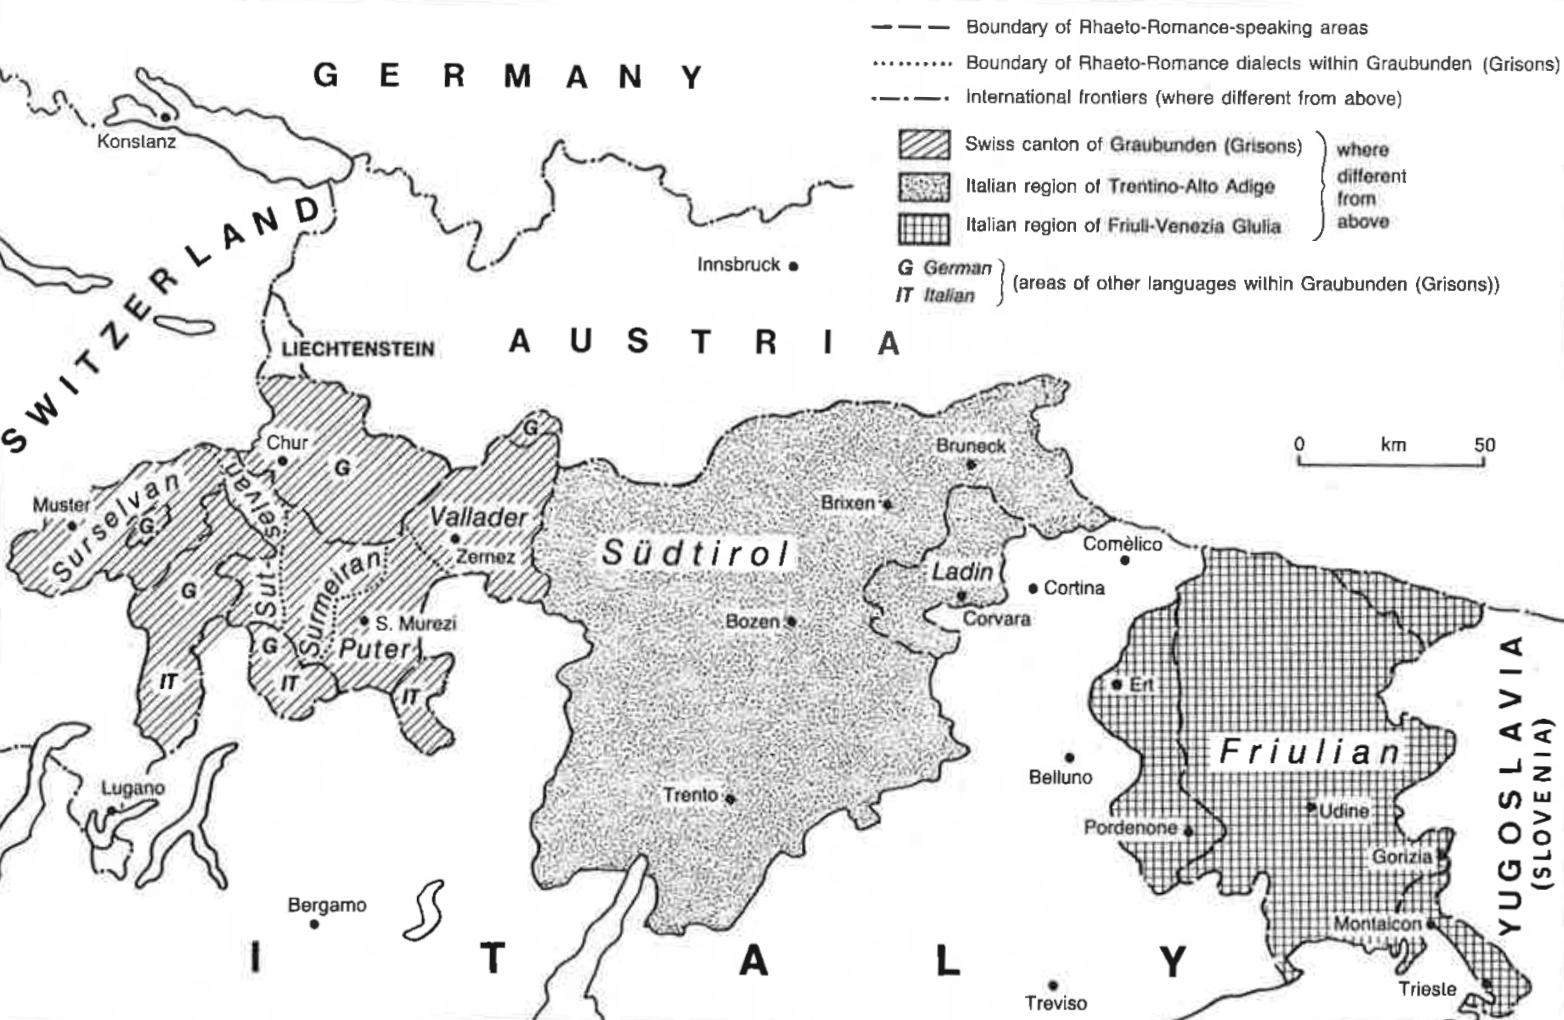
\includegraphics[width=0.8\textwidth]{graphics/raeto-map.png}
\caption[Map of the distribution of Rhaeto-Romance]{Distribution of Rhaeto-Romance, taken from \cite[2]{haiman1992}}
\label{fig:raeto-map}
\end{figure}

\section{Romansh}
The term Romansh is a collective name referring to the Rhaeto-Romance dialects spoken in Switzerland and are recognized as a single language. 
There are five different dialects (Surselvan, Sutselvan, Suermiran, Puter, Vallader), each having normative grammars and distinct orthographic norms (motivated by the Reformation, for translating the Bible and other religious texts) \autocites[1]{haiman1992}[178]{bossong2008}.

Romansh was officially acknowledged as a fourth official language in Switzerland (besides German, French and Italian) in a federal referendum that took place in 1938, in the eve of the Second World War, with a whopping majority of 92\% Yes votes. 
It has been hypothesized that this referendum played in the hands of the Rhaeto-Romans in \Gls{graubuenden} to promote their nationalistic political postulate, but was also instrumentalised by the Swiss federal government to counteract Mussolini's pretenses to \enquote{Italian} territories in Switzerland (referred to as the Italian irredentism\footnote{The nationalistic claim of lands inhabited by persons who the Italian nationalists saw as ethnic Italians.}) \autocite{valaer2012}.

Romansh is currently spoken by around 40,000 people \autocite{bundesamt2020}. 
This number has been diminishing constantly---30 years ago there were 50,000 speakers \autocite{haiman1992}. 
There is however hardly a single person who speaks only Romansh. 
In Switzerland, as in the other regions of Rhaeto-Romance, there is always a \enquote{prestige} language surrounding Rhaeto-Romance, in which Rhaeto-Romance speakers are fluent in \autocite[3]{haiman1992}. 

\section{Rumantsch Grischun}
\subsection{Lia Rumantscha}
In the past hundred years there has been a Rhaeto-Romance revival. 
In Switzerland, a major force in this language movement was the founding of the Lia Rumantscha (\enquote{The Romansh League}) in 1919, which was also a counter-force to the Italian irredentism\footnotemark[\value{footnote}]. 
It is an umbrella organization devoted to promoting and perserving the Rhaeto-Romance language and culture. Its goals include creating and promoting a common language awareness and identity among the Rhaeto-Romans. 
The organization is responsible for developing a language standard, as well as for language renovation, and generally representing the interests of the Romansh and its speakers, in Graubünden and in the Swiss diaspora \autocite{dazzi2012}.

\subsection{Rumantsch Grischun}
The endeavors of the Lia Rumantscha in the field of language planning and standardization led to the official launching of a pan-Romansh language---\emph{Rumantsch Grischun} \autocite[5]{haiman1992}. 
Its goal was not to replace the local dialects, but be available for persons, institutions, government agencies, companies etc., that want to use Romansh but require a language variant that would be inter-regional and intelligible by speakers of all dialects. The main motivation for planning an inter-regional standard was the failure of Romansh to establish itself as a fourth national language due to the lack of a written standard, despite the great willingness of the people.
The existence of a written standard was intended to make Romansh be better respected and incorporated in the canton of Graubünden, as well as on a federal level; 
it would also elevate its prestige in the eyes of its speakers \autocite{schmid1982}.

\subsection{Features}
Rumantsch Grischun was suggested in 1982 by the Zurich-born Romance linguist Heinrich Schmid. 
It was, however, not the first attempt to harmonize the Romansh dialects. 
In the 19th century, a high school teacher named Gion Antoni Bühler, made failed attempts to propagate for a \mbox{\emph{Romonsch fusionau}}; 
in the 1960's, a Swiss author from the canton of Graubünden, Leza Uffer, suggested \emph{Interrumantsch}, which was mainly based on the Surmiran dialect, but failed similarly \autocite[39]{liver1999}.

Rumantsch Grischun's success has been hypothesized to be mainly due to the favorable timing---the socioeconomical situation at the time as well as a change in the approach of many Rhaeto-Romans to their own language; but also due to the fact that Rumantsch Grischun, contrary to previous suggestions for a standard language, is more consistent and balanced between the dialects \autocite[69]{liver1999}. 
It never systematically favors one dialect over the other.

Without going too much into detail, Rumantsch Grischun favors the greatest common denominator by  taking the word forms common to the three most important written dialects (Sursilvan, Surmiran and Vallader). For instance, in all three dialects the word for \enquote{key} is \emph{clav}, hence, this is also the Rumantsch Grischun word for \enquote{key}.
In case the dialects do not agree, the word form common to the majority of dialects is taken, in a sort of \enquote{majority vote}. 
That way, one dialect over is never preferred over the others throughout. 

Clarity and transparency also play a major role. 
This means that forms which exhibit stem alternations, for instance between singular and plural, are abandoned in favor simpler, more regular forms.
Further, phenomenons that are specific to just one dialect are left out, such as the rounded front-vowels [y] and [ø] typical of the dialects of the Engadine, or the closing diphthong [\textsci w]\footnote{The diphthong starts with an open vowel [\textsci] and ends with a closed vowel [w], hence \enquote{closing}}, which is unique to Sursilvan \autocite[70]{liver1999}. 
See table~\ref{tab:rg-examples} for some examples.

This new language fulfills the requirements of its authors: it can be read and understood by any Rhaeto-Roman without them having to elaborately learn it and the differences to the specific dialects are minimal \autocite[72]{liver1999}. 


\begin{table}
\centering
\begin{tabular}{lllll}
\toprule
Sursilvan & Surmiran & Vallader & Rumantsch Grischun & Principle \\
\midrule
\textbf{clav}	  &  \textbf{clav}    &  \textbf{clav}    & \textbf{clav}  \enquote{key}  & Greatest common denominator \\
\textbf{tschiel}       &   \textbf{tschiel}   & tschel      & \textbf{tschiel} \enquote{sky} & Majority vote \\
siat 	 & \textbf{set}      & \textbf{set}      & \textbf{set} \enquote{seven} & " \\
\textbf{cor} & \textbf{cor} & cour & \textbf{cor} \enquote{heart} & " \\
vendiu & vendia & vendü & \textbf{vendi} \enquote{bought} & Favor simplicity \\
sg./pl. \emph{iert}/\emph{orts} & \textbf{iert/ierts} & üert/üerts & iert/ierts \enquote{garden} & " \\
\bottomrule

\end{tabular}
\caption[Examples for choosing the forms for Rumanstch Grischun]{Examples for choosing the forms for Rumanstch Grischun, based on \cite[70-71]{liver1999}}
\label{tab:rg-examples}
\end{table}


\subsection{Today}
Rumantsch Grischun has become one of the most ambitious endeavours in the history of Romansh. 
Since its invention, Romansh and the people promoting it have had notable success achieving their goals. 
In 1999, Romansh became a \enquote{partially official language} (\emph{Teilamtssprache}) of the Swiss confederation. 
In 2003, it was recognized in the cantonal constitution of Graubünden as an equal cantonal language, and the protection of the traditional language regions was guaranteed.
Nowadays, Romansh is in use in many domains, not only in the public administration, but also in economy. 
Many writings and works were written in Rumantsch Grischun. 
People learn to read and write in Rumantsch Grischun and in some schools, classes are held in it. 
The extent of radio and television in Romansh has been growing. 
There is a radio station broadcasting 24/7, television programs in Romansh are broadcast in all public channels of the Swiss Broadcating Corporation (SSG SSR), and there are also internet portals, e.g., \url{https://www.rtr.ch/}. All of this wouldn't have been possible if it weren't for the political \enquote{upgrade} that was aspired for by the Romansh language movement \autocite{cathomas2012}.

The canton of Graubünden has been releasing most or all of its press releases since 1998 in three languages: German, Italian and Romansh using the Rumantsch Grischun standard. 
I therefore decided to collect these press releases and use them to compile a parallel corpus. 

From this point on, the term \emph{Romansh} will refer to the standard variant \emph{Rumantsch Grischun}.